\documentclass[]{book}
\usepackage{lmodern}
\usepackage{amssymb,amsmath}
\usepackage{ifxetex,ifluatex}
\usepackage{fixltx2e} % provides \textsubscript
\ifnum 0\ifxetex 1\fi\ifluatex 1\fi=0 % if pdftex
  \usepackage[T1]{fontenc}
  \usepackage[utf8]{inputenc}
\else % if luatex or xelatex
  \ifxetex
    \usepackage{mathspec}
  \else
    \usepackage{fontspec}
  \fi
  \defaultfontfeatures{Ligatures=TeX,Scale=MatchLowercase}
\fi
% use upquote if available, for straight quotes in verbatim environments
\IfFileExists{upquote.sty}{\usepackage{upquote}}{}
% use microtype if available
\IfFileExists{microtype.sty}{%
\usepackage{microtype}
\UseMicrotypeSet[protrusion]{basicmath} % disable protrusion for tt fonts
}{}
\usepackage{hyperref}
\hypersetup{unicode=true,
            pdftitle={Análise do impacto da formação em Medicina de Família e Comunidade na reforma da atenção primária à saúde no Rio de Janeiro},
            pdfauthor={Adelson Guaraci Jantsch},
            pdfborder={0 0 0},
            breaklinks=true}
\urlstyle{same}  % don't use monospace font for urls
\usepackage{natbib}
\bibliographystyle{apalike}
\usepackage{longtable,booktabs}
\usepackage{graphicx,grffile}
\makeatletter
\def\maxwidth{\ifdim\Gin@nat@width>\linewidth\linewidth\else\Gin@nat@width\fi}
\def\maxheight{\ifdim\Gin@nat@height>\textheight\textheight\else\Gin@nat@height\fi}
\makeatother
% Scale images if necessary, so that they will not overflow the page
% margins by default, and it is still possible to overwrite the defaults
% using explicit options in \includegraphics[width, height, ...]{}
\setkeys{Gin}{width=\maxwidth,height=\maxheight,keepaspectratio}
\IfFileExists{parskip.sty}{%
\usepackage{parskip}
}{% else
\setlength{\parindent}{0pt}
\setlength{\parskip}{6pt plus 2pt minus 1pt}
}
\setlength{\emergencystretch}{3em}  % prevent overfull lines
\providecommand{\tightlist}{%
  \setlength{\itemsep}{0pt}\setlength{\parskip}{0pt}}
\setcounter{secnumdepth}{5}
% Redefines (sub)paragraphs to behave more like sections
\ifx\paragraph\undefined\else
\let\oldparagraph\paragraph
\renewcommand{\paragraph}[1]{\oldparagraph{#1}\mbox{}}
\fi
\ifx\subparagraph\undefined\else
\let\oldsubparagraph\subparagraph
\renewcommand{\subparagraph}[1]{\oldsubparagraph{#1}\mbox{}}
\fi

%%% Use protect on footnotes to avoid problems with footnotes in titles
\let\rmarkdownfootnote\footnote%
\def\footnote{\protect\rmarkdownfootnote}

%%% Change title format to be more compact
\usepackage{titling}

% Create subtitle command for use in maketitle
\providecommand{\subtitle}[1]{
  \posttitle{
    \begin{center}\large#1\end{center}
    }
}

\setlength{\droptitle}{-2em}

  \title{Análise do impacto da formação em Medicina de Família e Comunidade na reforma da atenção primária à saúde no Rio de Janeiro}
    \pretitle{\vspace{\droptitle}\centering\huge}
  \posttitle{\par}
    \author{Adelson Guaraci Jantsch}
    \preauthor{\centering\large\emph}
  \postauthor{\par}
      \predate{\centering\large\emph}
  \postdate{\par}
    \date{2020-01-02}

\usepackage{booktabs}

\begin{document}
\maketitle

{
\setcounter{tocdepth}{1}
\tableofcontents
}
\hypertarget{section}{%
\chapter*{}\label{section}}
\addcontentsline{toc}{chapter}{}

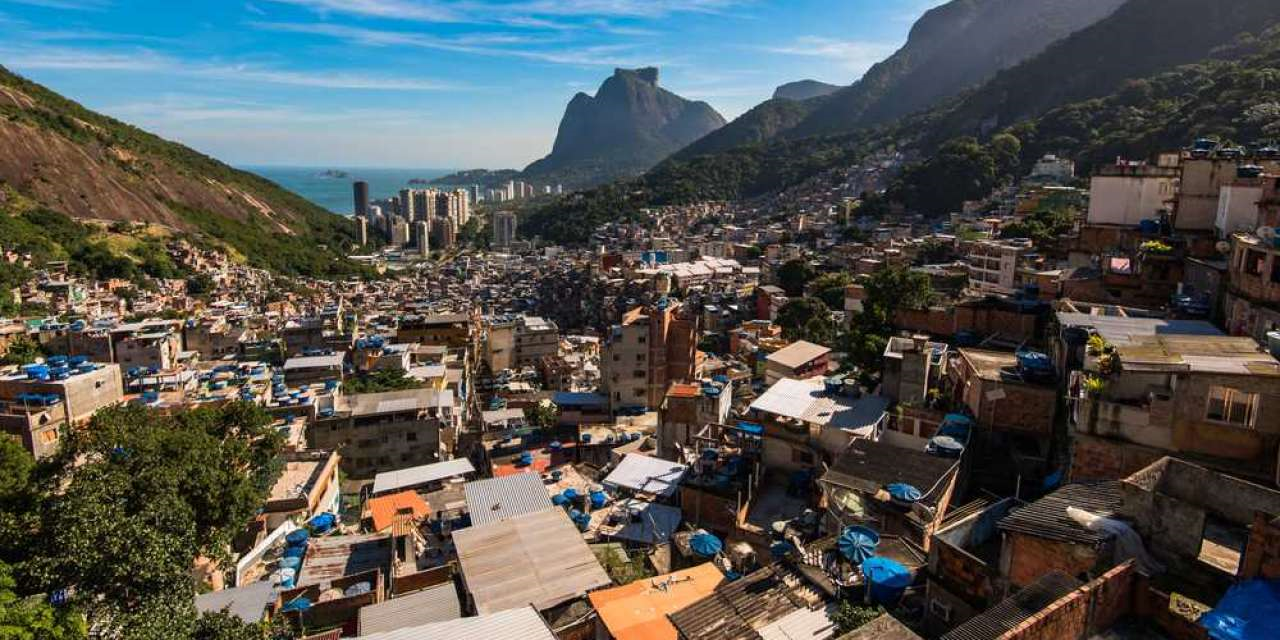
\includegraphics{C:/Users/Adelson/Desktop/thesis/subindo/family_medicine_impact/livro/rocinha.png}

\hypertarget{introduction}{%
\chapter*{Introduction}\label{introduction}}
\addcontentsline{toc}{chapter}{Introduction}

\begin{verbatim}
Mas eu ainda espero angariar as simpatias da opinião, 
e o primeiro remédio é fugir a um prólogo explícito e longo.
\end{verbatim}

Perguntar se investimento em educação é benéfico para a sociedade pode parecer algo obsoleto e desnecessário. Qualquer pessoa com o mínimo de instrução e bom senso concordaria que educação é um dos pilares que estruturam as sociedades e que investir recursos financeiros nesta área é fundamental para o seu desenvolvimento. Essas afirmações fazem parte da retórica política corrente e aparentemente não há discordância quanto à importância da universalização da alfabetização, da aquisição de conhecimentos gerais, do desenvolvimento de habilidades matemáticas, do conhecimento de história, geografia e ciências. Contudo, há uma série de fatos históricos, políticos e econômicos que tornam a discussão sobre ensino médico e treinamento de especialidades uma questão um pouco mais complexa do que se pode supor.

Apesar de ter o primeiro programa de residência iniciado em 1944 no Brasil, a regulamentação desta forma de curso de pós-graduação latu sensu veio a acontecer somente em 19771 a partir do decreto nº 80.281 que criava a Comissão Nacional de Residências Médicas (CNRM) e estabelecia que os programas de residência médica seriam caracterizados por ``treinamento em serviço, em regime de dedicação exclusiva, funcionando em Instituições de saúde, universitárias ou não, sob a orientação de profissionais médicos de elevada qualificação ética e profissional'' e que teriam duração mínima de um ano, contemplando 1.800 horas de atividade assistencial, sendo quatro horas semanais dedicadas a atividades de teóricas não assistenciais2. Isso ocorreu antes do estabelecimento do Sistema Único de Saúde3 (SUS) e antes mesmo do estabelecimento da Medicina de Família ser reconhecida como especialidade médica, fato que ocorreu em 1981 ainda sob o nome de Medicina Geral e Comunitária4.

Apesar do aumento recente na oferta de vagas para residência médica no Brasil impulsionado pelo pelo Programa PróResidência5 que aumentou a oferta de vagas em áreas prioritárias do país, em 2017 havia somente 16.499 vagas ofertadas para um contingente de 18.753 novos médicos formados6. Além de oferta ainda limitada de vagas para atender à demanda de médicos recém-formados, há também problemas quanto à distribuição destas vagas de acordo com as especialidades médicas, sendo a Atenção Primária à Saúde (APS) a área mais sensível à esta distribuição desigual. Por ser um nível de atenção à saúde ainda em construção no Brasil, apresenta uma demanda enorme de Médicos de Família e Comunidade treinados e capacitados, porém apenas 4,4\% das vagas atuais de residência são destinadas a esta especialidade7.

Formação médica especializada no formato de residência médica, ainda não é universal para todos os alunos graduados em escolas médicas no Brasil e comumente um aluno recém formado pode não conseguir uma vaga de residência na especialidade escolhida mesmo prestando prova para diversos programas. Ao mesmo tempo em que vários médicos recém-formados ficam de fora de programas de residência médica pela falta de vagas, a legislação brasileira permite ao médico trabalhar e exercer procedimentos específicos mesmo sem nenhuma especialização formal e reconhecida8,9. Isto é algo que aproxima o Brasil a outros países de baixa e média renda quanto a governança e regulação e o afasta daqueles onde a APS encontra-se madura nos quais uma grande parte das vagas são destinadas para Medicina de Família.

Dentro de um cenário hospitalar, em um ambiente cirúrgico, dificilmente um cirurgião sem especialização em cirurgia cardíaca seria contratado para realizar uma valvuloplastia, por exemplo, mas não é incomum que médicos sem treinamento exerçam a função de emergencistas -- função comumente exercida por médicos recém-formados no Brasil e que não recebe a mesma importância dada em alguns países desenvolvidos. Neste contexto, as forças que orientam e regulam a oferta de vagas em residência médica, os tipos de especialidades que serão privilegiadas e os locais de aberturas de novas vagas de residência não são orientadas exclusivamente visando atender às demandas de saúde da população, mas recebem grande influência de grupos políticos de especialidades e corporações médicas2.

Apesar da falta de regulação e de planejamento estratégico na formação médica especializada para atender às demandas em saúde da população e de termos uma desigualdade enorme na densidade de médicos no país, concentrando especialistas nos grandes centros urbanos e áreas mais ricas, as políticas de incentivo para a criação de novas vagas de residência médica privilegiaram a MFC, aumentando de 1,4\% para 4,4\% das vagas ofertadas no país6. Mesmo assim, a proporção de vagas de residência em MFC no Brasil ainda é muito menor do que o encontrado em países como Canadá, Espanha e Inglaterra, onde metade do total de vagas é destinado à MFC10. Isso deixa o Brasil muito distante de alcançar a meta regional estabelecida pela Organização Panamericana de Saúde de que 40\% da força laboral deve estar concentrada na APS11. A obrigatoriedade de cursar um programa de residência para se exercer a medicina ainda está longe de se tornar uma realidade no Brasil, fazendo com que provimento, fixação e desenvolvimento de competências clínicas - três objetivos principais da formação médica especializada - continuem sendo metas muito longe de serem alcançadas2.

Nos seus quase 30 anos de história o Sistema Único de Saúde (SUS), com suas diretrizes de universalidade, integralidade do cuidado, participação popular, resolutividade e equidade3, conseguiu avanços importantes ao ampliar acesso a serviços e garantindo direito ao cuidado em saúde. Contudo, muito ainda precisa ser feito para que seja considerado um sistema de saúde robusto e verdadeiramente universal, principalmente minimizando desigualdades em saúde entre regiões ricas e pobres do país12.

Além das dificuldades históricas de desenvolvimento do sistema de saúde, eventos recentes trazem uma ameaça séria à sustentabilidade do SUS, a partir da implementação das políticas de austeridade propostas durante os anos de governo de Michel Temer13, colocando em risco conquistas importantes alcançadas durante sua história, como ampliação da APS, aumento da cobertura de serviços, redução da mortalidade infantil14 e da mortalidade por doenças crônicas não transmissíveis (DCNT)15. Com a implementação das políticas de austeridade e com o previsto congelamento de investimentos na área da saúde e educação pelos próximos 20 anos há expectativa de uma redução na diminuição da taxa de mortalidade infantil, fazendo com que o país reduza os ganhos que seriam esperados em saúde caso os investimentos fossem mantidos16.

Historicamente algumas iniciativas buscaram minimizar essas desigualdades de acesso a serviços e a primeira estratégia nacional voltada para a atenção primária à saúde (APS) foi o Programa de Saúde da Família (PSF) que, desde sua concepção em 1991 e implementação em 199417, ampliou gradativamente sua cobertura de população assistida, chegando a 56\% de cobertura em 201318, e a 64\% em 201619. Esta iniciativa teve impactos substanciais sobre a saúde da população brasileira, principalmente na redução da mortalidade infantil20, na redução de internações hospitalares desnecessárias21 e na redução da mortalidade por doenças cardiovasculares22.

Contudo, não foi somente em indicadores de saúde pública que este programa teve efeito. A criação de novos postos de trabalho em unidades de APS teve também um efeito tanto no mercado de trabalho, ao aproximar novos médicos do trabalho na APS, impulsionando assim o crescimento da Sociedade Brasileira de Medicina de Família SBMFC), quanto na criação de um novo mercado de trabalho nos planos privados de saúde, que passaram a ver a MFC como uma forma de trazer os atributos da APS para seus seus serviços, reduzindo custos e trazendo melhores resultados no cuidado em saúde23,24.

\hypertarget{literature}{%
\chapter*{Literature}\label{literature}}
\addcontentsline{toc}{chapter}{Literature}

The Brazilian PHC system started in 1991 with the community health agents program and scaled up to the Family Health Program in 1994 when the initiative as a federal policy stablished a structure for PHC at the municipal level, providing financial resources for a Family Health Team (FHT) formed by one Physician, one Nurse and 4 to 6 Community Health Agents to take care of 4000 people living inside a catchment area. In Rio de Janeiro a PHC reform took place between 2009 and 2016115 when the Health Department created new community-based PC clinics and new FHT, increasing the coverage from 3.5\% to almost 70\% of the population of the city. Currently 1400 FHT are working in the city, providing care for more than 3.5 million people in a system that merges public funding with private non-for-profit organizations responsible for management and for structural and human resources.

\hypertarget{methods}{%
\chapter*{Methods}\label{methods}}
\addcontentsline{toc}{chapter}{Methods}

We describe our methods in this chapter.

\hypertarget{the-rio-de-janeiro-practice-based-research-network-database---real-world-information-to-study-primary-care-and-family-medicine.}{%
\chapter*{The Rio de Janeiro practice-based research network database - real world information to study primary care and family medicine.}\label{the-rio-de-janeiro-practice-based-research-network-database---real-world-information-to-study-primary-care-and-family-medicine.}}
\addcontentsline{toc}{chapter}{The Rio de Janeiro practice-based research network database - real world information to study primary care and family medicine.}

\hypertarget{introduction-1}{%
\section*{Introduction:}\label{introduction-1}}
\addcontentsline{toc}{section}{Introduction:}

For the last 40 years, many advances in Primary Health Care (PHC) were made due to the momentum created by the Alma-Ata declaration35. Many countries have achieved good results in creating and developing universal, accessible, and cost-effective PHC systems25,107. The principles stated in 1978 in Alma-Ata were reinforced in 2018 by the Astana declaration108, pointing the importance of having a strong PHC as a strong element of social development to achieve social justice and good health.

With short and strong sentences, these documents state that health disparities will only be overcome through strong PHC built in a spirit of social justice relying on health workers that are ``suitably trained socially and technically to work as a health team'' and to ``respond to the expressed health needs of the community''35. The big picture is clear, but having a closer look at the terms ``health workers'' and ``health teams'' we cannot find any specification about what should be the health workers in PHC or how a health team must be assembled. Many times family physicians (FP) use the terms PHC and Family Medicine (FM) interchangeably -- maybe because they work in primary care, maybe because they see themselves as the specialists in primary care -- but in those documents FM is never mentioned as the medical specialty for primary care.

Only at the World Health Report 200839 the World Health Organization mention FM referring to the fact that PHC has been studied extensively in high income countries where physicians with specialization in FM working in PC is the norm. This is a very important fact related to the development of PHC -- and FM -- around the world. In many low and middle income countries (LMIC) FM is not even a medical specialty10 and, when it is present, the role FP play as health care providers can vary largely depending on the health system109. The lack of a globally accepted definition is a consequence of the incipiency of the specialty in LMIC110. For those countries the question of proving the value of having a strong PHC system for policymakers and health managers is part of the daily struggle for sustainability - the same can be said about FM.

Studies looking at the impact of PHC often miss this important element involved in delivering care for the patients, that is the medical professional. In Brazil, a country with a large universal public health care system111 and a successful history of development of community-based primary care15, studies about its impact have proven substantial effects on reducing infant and neonatal mortality112, hospital admissions related to ambulatory-care sensitive conditions113 and cardiovascular deaths22, but also fail to address the impact of the medical specialty.

Under the national Programa de Saúde da Família (Family Health Program - FHP) launched in 1994, Family Health Teams (FHT) composed by one doctor, one nurse and four to six community health agents provide care for 4,000 people in a catchment area. Today, 64\% of the Brazilian population is covered by the 43,000 FHT active in the programe19, but only a few of those teams have a trained family physician as the doctor in charge. Despite recent policies that have tried to boost28,114 the creation and growth of residency programs in FM, only 4.4\% of the residency training seats are dedicated to FM. With only 5,500 FP in the country6 (1.4\% of all specialists; not all of them with residency training), FM is still not seen by policymakers and health managers as a necessary medical specialty to be a health care provider in PHC.

One recent exception was the PHC reform experienced in Rio de Janeiro from 2008 until 2016, when the coverage of the PSF increased from 3.5\% to almost 70\% and investments were made to create a new FM training program in 2012 (and expand the two programs already stablished) as a capacity building initiative for human resources115. 206 seats are offered every year for doctors who want to become FP. They attend a two-year program with a workload of 55 hours per week, 90\% of them in community-based primary care clinics, with a strong emphasis in clinical reasoning, communication skills, patient-centered care, multimorbidity and patients' complexity, evidence-based medicine, quality improvement activities, research in PC, training of small procedures, care of vulnerable and neglected populations and clinical content about the most prevalent conditions in primary care116. They receive monthly a standard scholarship for two years from the ministry of health (R\$ 3,300.00 or US\$ 820 - same for every resident in Brazil), and an extra scholarship (R\$ 7,000.00 or US\$ 1,740) from the municipality, as a financial incentive for provision and fixation. Preceptors (trainers) also receive a financial incentive for being responsible for supervising two to four residents31.

Today Rio de Janeiro alone is responsible for almost 20\% of the FM training seats in the country and almost 85\% of the graduted students end up working at the public PHC system in Rio de Janeiro. This initiative created a natural experiment in the city, where some FHT have a FP as the doctor in charge, others have doctors with only a medical degree and no residency training (generalists). A perfect setting for studies about the effect of family medicine training on patient care in PHC.

The Rio de Janeiro practice-based research neetwork (RioPBRN) is the novice research unit created by the Family and Community Medicine Residency Program at the Rio de Janeiro Health Department. Nowadays it has been building a data-warehouse compiling information related to primary care in Rio de Janeiro that will serve as data source for researchers interested on PHC subjects, such as training in FM and capacity building of human resources, PHC in LMIC, health care systems development, cost-effectiveness analysis, community-based primary care and team-based work. This article aims to present the structure of this dataset and the story behind the process of building it.

\hypertarget{quick-references}{%
\chapter*{Quick references}\label{quick-references}}
\addcontentsline{toc}{chapter}{Quick references}

\hypertarget{clinical-governance}{%
\section*{Clinical governance}\label{clinical-governance}}
\addcontentsline{toc}{section}{Clinical governance}

\begin{itemize}
\tightlist
\item
  Look at page 25 - \href{https://www.ncbi.nlm.nih.gov/pmc/articles/PMC1113460/pdf/61.pdf}{Clinical governance and the drive for quality improvement in the new NHS in England}
\end{itemize}

\hypertarget{sus}{%
\section*{SUS}\label{sus}}
\addcontentsline{toc}{section}{SUS}

\begin{itemize}
\tightlist
\item
  From 2000 to 2014, total health expenditure rose from 7.0\% to 8.3\% of gross domestic product and population coverage with the Family Health Strategy rose from 7.6\% to 58.2\%. \href{https://www.ncbi.nlm.nih.gov/pmc/articles/PMC6035510/pdf/bmjgh-2018-000829.pdf}{The Brazilian health system at crossroads: progress, crisis and resilience}
\end{itemize}

\hypertarget{capacity-building-of-human-resources}{%
\section*{Capacity building of Human resources}\label{capacity-building-of-human-resources}}
\addcontentsline{toc}{section}{Capacity building of Human resources}

\begin{itemize}
\item
  Programa Nacional de Apoio à Formação de Médicos Especialistas em Áreas Estratégicas -- Pró-Residência, criado em 2009 \href{http://www.scielo.br/pdf/physis/v26n2/0103-7331-physis-26-02-00633.pdf}{Regulação da formação de especialistas: inter-relações com o Programa Mais Médicos}
\item
  \href{Pró-Residência}{Formação de Médicos Especialistas no SUS: Descrição e Análise da Implementação do Programa Nacional de Apoio à Formação de Médicos Especialistas em Áreas Estratégicas}{]}(\url{http://www.scielo.br/pdf/rbem/v37n1/11.pdf})\{target="\_blank"\}
\end{itemize}

\hypertarget{evidences-about-primary-care-in-brazil}{%
\section*{Evidences about primary Care in Brazil}\label{evidences-about-primary-care-in-brazil}}
\addcontentsline{toc}{section}{Evidences about primary Care in Brazil}

\begin{itemize}
\item
  \href{https://www.healthaffairs.org/doi/full/10.1377/hlthaff.2016.0966?url_ver=Z39.88-2003\&rfr_id=ori:rid:crossref.org\&rfr_dat=cr_pub\%3dpubmed}{Large reductions in amenable mortality associated with Brazil's Primary Care expansion and strong health governance. Health Affairs, 36(1), 149--158. Hone, T., Rasella, D., Barreto, M., Atun, R., Majeed, A., \& Millett, C. (2017). doi:10.1377/hlthaff.2016.0966}
\item
  Statistically significant associations were found between indicators of ESF coverage and presence of SAMU with indicators of stroke and AMI mortality, for both sexes, except for male AMI. \href{http://www.scielo.br/pdf/ramb/v56n4/en_19.pdf}{Analysis of prehospital care for stroke and acute myocardial infarction in the elderly population of Minas Gerais, Brazil}
\item
  A recomendação para outra pessoa dos serviços de saúde utilizados foi mais frequente entre usuários regulares da ESF (61,9\%) e afiliados a plano privado (55,6\%), em comparação à UBS (45,4\%). \href{http://www.scielo.br/scielo.php?script=sci_arttext\&pid=S0102-311X2013000700011\&lng=en\&nrm=iso\&tlng=en}{Estratégia Saúde da Família em comparação a outras fontes de atenção: indicadores de uso e qualidade dos serviços de saúde em Belo Horizonte, Minas Gerais, Brasil}
\end{itemize}

\hypertarget{family-medicine}{%
\section*{Family Medicine}\label{family-medicine}}
\addcontentsline{toc}{section}{Family Medicine}

\begin{itemize}
\tightlist
\item
  \href{https://www.ncbi.nlm.nih.gov/pmc/articles/PMC5471080/pdf/0630436.pdf}{Family medicine around the world: overview by region The Besrour Papers: a series on the state of family medicine in the world} Neil Arya, Christine Gibson, David Ponka, Cynthia Haq, Stephanie Hansel, Bruce Dahlman, Katherine Rouleau
\end{itemize}

\hypertarget{family-medicine-and-public-health}{%
\section*{Family Medicine and Public Health}\label{family-medicine-and-public-health}}
\addcontentsline{toc}{section}{Family Medicine and Public Health}

\begin{itemize}
\item
  Explaining what is general practice and public health. General practitioners (GPs) tend to focus most of their energies on providing primary healthcare to individuals, with less attention to the overall population health issues in their community. In contrast, public health practitioners tend to focus on the health needs of entire populations, by addressing the social determinants of health, with less attention to individual patient care.
  \href{https://www.racgp.org.au/afp/2014/july/who-is-my-patient/}{General practice and public health: who is my patient? Volume 43, No.7, July 2014 Pages 483-486}
\item
  About super specialization in the US - \href{https://www.amjmed.com/article/S0002-9343\%2817\%2930134-1/pdf}{Where Have the Generalists Gone? They Became Specialists, Then Subspecialists}
\end{itemize}

\hypertarget{ambulatory-care-sensitive-conditions}{%
\section*{Ambulatory-care sensitive conditions}\label{ambulatory-care-sensitive-conditions}}
\addcontentsline{toc}{section}{Ambulatory-care sensitive conditions}

\begin{itemize}
\item
  Primeiro artigo a citar o termo ambulatory-care sensitive conditions \href{https://www.healthaffairs.org/doi/pdf/10.1377/hlthaff.12.1.162}{Impact Of Socioeconomic Status On Hospital Use In New York City} John Billings, Lisa Zeitel, Joanne Lukomnik, Timothy S. Carey, Arthur E. Blank, and Laurie Newman
\item
  \href{http://www.scielo.br/pdf/csp/v25n6/16.pdf}{Internações por condições sensíveis à atenção primária: a construção da lista brasileira como ferramenta para medir o desempenho do sistema de saúde (Projeto ICSAP -- Brasil)}
\item
  Sensitive conditions accounted for 115,340 (26.4\%) hospitalizations. Over the 4-year period, hospitalizations for sensitive conditions declined by 17.9\%, vs only 8.3\% for non-sensitive ones (P\textless{}0.001). Hospitalization for sensitive conditions declined 22\% for women in areas of high social vulnerability vs 9\% for women in areas of low vulnerability (P\textless{}0.001); for men, 17\% vs 10\% (P=0.11). \href{https://academic.oup.com/heapol/article/27/4/348/605470}{Trends in hospitalizations for primary care sensitive conditions following the implementation of Family Health Teams in Belo Horizonte, Brazil, Claunara Schilling Mendonça, Erno Harzheim, Bruce B Duncan, Luciana Neves Nunes, Werner Leyh}
\item
  \href{http://www.scielo.br/scielo.php?script=sci_arttext\&pid=S1414-462X2018000200178\&lng=pt\&nrm=iso\&tlng=pt}{Internações por condições sensíveis à atenção primária à saúde, 2008-2015: uma análise do impacto da expansão da ESF na cidade do Rio de Janeiro}\\
  Identificou-se tendência ao aumento da cobertura da ESF e à redução dos indicadores de ICSAP, bem como correlação inversa entre a cobertura pela ESF e a proporção de ICSAP (r = -0,888, p = 0,020), e entre a cobertura pela ESF e a taxa de ICSAP (r = -0,753, p = 0,031). Observou-se associação significativa para as razões de taxa dos indicadores de cobertura a partir de 2011 e de taxas de internação a partir de 2013.\\
  Cad. saúde colet. vol.26 no.2 Rio de Janeiro abr./jun. 2018 \url{http://dx.doi.org/10.1590/1414-462x201800020230}
\item
  ACSC hospitalization, while being a negative index of primary care access, can also be a measure indicating the impact of the hospital bed supply, and it is still a valid measure of the disparity of health care, the original motivation for this topic. \href{https://bmchealthservres.biomedcentral.com/articles/10.1186/s12913-019-4098-x}{Hospitalizations for ambulatory care sensitive conditions as an indicator of access to primary care and excess of bed supply}
\end{itemize}

\hypertarget{cash-transfer-programs}{%
\section*{Cash transfer programs}\label{cash-transfer-programs}}
\addcontentsline{toc}{section}{Cash transfer programs}

\begin{itemize}
\tightlist
\item
  \href{https://sci-hub.tw/https://doi.org/10.1016/S0140-6736(13)60715-1}{Effect of a conditional cash transfer programme on childhood mortality: a nationwide analysis of Brazilian municipalities}
\end{itemize}

\bibliography{book.bib,packages.bib}


\end{document}
